\begin{frame}{Un héritage}
  Vous venez de savoir que vos partenaires ont récemment héritié d'une grande somme d'argent.
  Réfléchissez à des questions que vous voudriez leur poser.
  Écrivez une question pour chaque pronom interrogatif suivant.
  Par exemple: \\
  \begin{itemize}
    \item \emph{Qui est-ce qui va te demander de l'argent?}
  \end{itemize}
  \begin{columns}
    \column{0.5\textwidth}
      \only<1>{
        \begin{enumerate}
          \item qu'est-ce que
          \item qu'est-ce qui
          \item qui est-ce que
          \item qui est-ce qui
        \end{enumerate}
      }
      \only<2>{
        Maintenant, posez vos questions à des partenaires, et discutez des réponses.
      }
    \column{0.5\textwidth}
      \begin{center}
        \scriptsize
        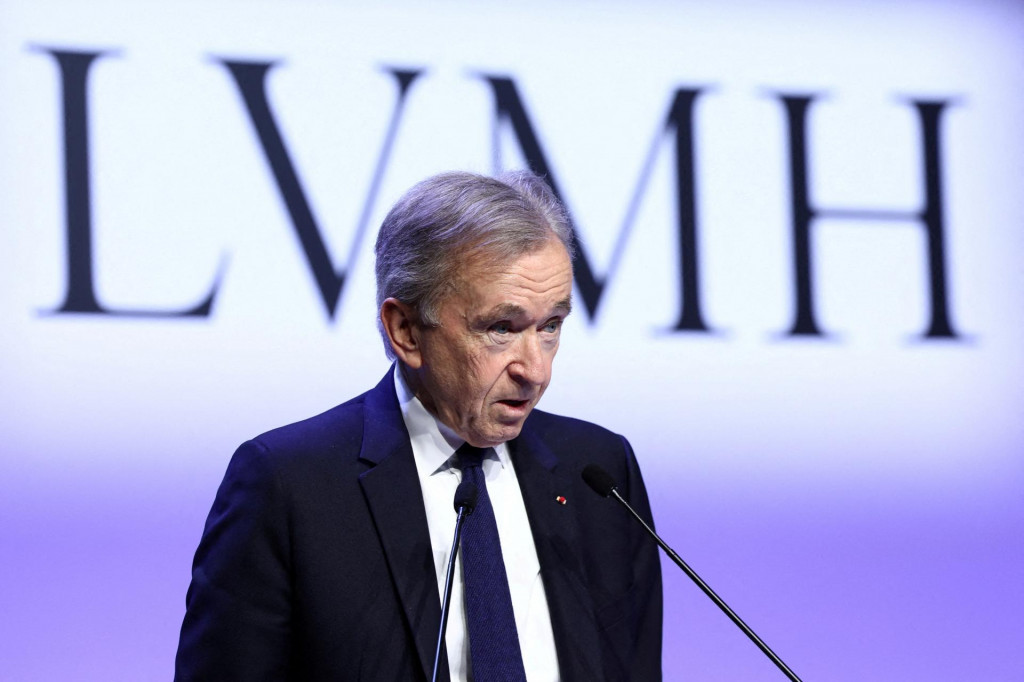
\includegraphics[scale=0.18]{bernard_arnault.jpg} \\
        Bernard Arnault de France \\
        Une fortune estimée \\
        à 233 milliards de dollars en 2024
      \end{center}
  \end{columns}
\end{frame}